\section{Hardware Platform}
\label{sec:back:hw}

This project targets the EFM32GG \gls{mcu} developed by Silicon Labs.
The following sections presents the EFM32 family of microcontrollers and a couple of development kits that utilize the Giant Gecko \gls{mcu}, soldered with a handful of different peripherals.

\subsection{EFM32}
\label{sub:emf32}

ARM Cortex-M is a family of 32-bit RISC processor cores, intended to be used by applications that require low cost and energy-usage.
These factors are crucial in modern systems and applications where energy efficiency is of great importance.
For example with the \gls{iot} \cite{Valhouli2010}, where it is predicted that tens of billions of devices will be connected to the Internet in the future, ranging from Super Computers down to small embedded devices that might be used to power up and control everything from cars to light bulbs via the Internet.
The different processor cores of the Cortex-M family are summarized in \autoref{tab:cortex_m}.

\begin{table}[h]
\begin{center}
\begin{tabular}{r|l}
    \textbf{Name} & \textbf{Target features}            \\
    \hline
    Cortex-M0 & Lowest cost and lowest area              \\
    Cortex-M0+ & Lowest power                            \\
    Cortex-M1 & Designed for implementation in FPGAs     \\
    Cortex-M3 & Performance efficiency                   \\
    Cortex-M4 & DSP, SIMD, FP                            \\
    Cortex-M7 & Cache, TCM, AXI, ECC, double + single FP \\
    \hline
    \end{tabular}
\end{center}
\caption{Cortex-M family of processor cores}
\label{tab:cortex_m}
\end{table}

The EFM32 family of microcontrollers are all based on different Cortex-M processors, some of their features are summarized in \autoref{tab:efm32_family}.
The focus of these microcontrollers is energy efficiency and low power-consumption in resource-constraint environments.
The EFM32GG, usually referred to with the name \chip{Giant Gecko}, is a versatile chip that is in the upper end in the Cortex-M series.
This is the processor core that is targeted in this project, and for the sake of simplicity we will refer to this chip as the {\gecko}.

The microcontrollers implement several different methods for reducing the power consumption.
The most important way to achieve low power consumption is by turning off the different parts of the chip that are inactive, so that these parts do no longer draw any power from the overall system.
The EFM32 processors features five different energy modes, or sleep modes, ranging from EM0 (Energy Mode 0) where the core is on, to EM4 where the processor can only wake up on specific interrupt signals.
The different peripherals provided with the EFM32's operate in different energy modes.
This system allows applications to utilize many different peripherals for data collection, while the processor itself is turned off.
The peripherals then have the opportunity to wake up the processor on different interrupt-signals and transfer data to it, in order to do general processing.

\begin{table}[b]
\begin{center}
    \begin{tabular}{r|l|l|l}
    \textbf{Name} & \textbf{Processor} & \textbf{Speed (MHz)} & \textbf{Flash Memory (KB)} \\
    \hline
    Zero Gecko    & ARM Cortex-M0+ & 24 & 4, 8, 16, 32    \\
    Tiny Gecko    & ARM Cortex-M3  & 32 & 4, 8, 16, 32    \\
    Gecko         & ARM Cortex-M3  & 32 & 16, 32, 64, 128 \\
    Leopard Gecko & ARM Cortex-M3  & 48 & 64, 128, 256    \\
    Giant Gecko   & ARM Cortex-M3  & 48 & 512, 1024       \\
    Wonder Gecko  & ARM Cortex-M4  & 48 & 64, 128, 256    \\
    \hline
    \end{tabular}
\end{center}
\caption{EFM32 Product Family \cite{Labs2014}.}
\label{tab:efm32_family}
\end{table}

\subsection{Evaluation boards}

Silicon Labs provides a wide range of development-kits and -boards that are targeted for general development and testing of applications based on the EFM32's.
Two of these boards are available with the {\gecko} and we have used both of them in this project.
The simplest of the two are the \chip{Giant Gecko} Starter Kit, which is depicted in \autoref{fig:efm32gg-stk3700}.
This board contains a few LEDs and buttons, a couple of sensors to demonstrate a wide range of use-cases, and a segment LCD display.
It also includes an expansion header that can be used to connect with third party devices and peripherals, and a JLink debug interface over USB.

\begin{figure}[H]
  \begin{center}
    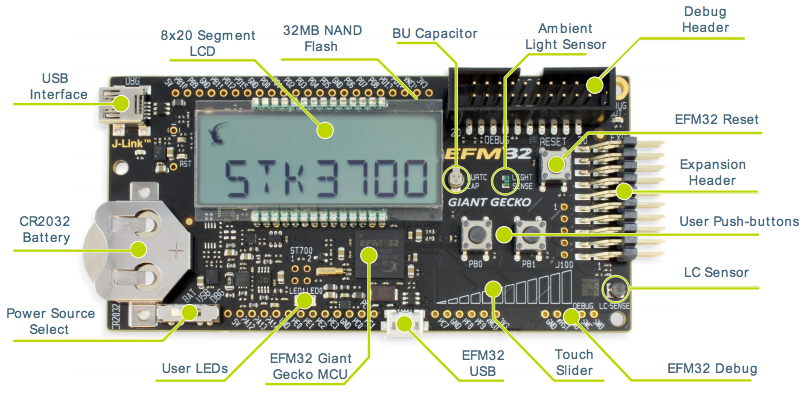
\includegraphics[scale=0.4]{figures/efm32gg-stk3700}
  \end{center}
  \caption{The Giant Gecko Starter Kit - EFM32GG-STK3700 \cite{Labs2013_STK} }
  \label{fig:efm32gg-stk3700}
\end{figure}

As seen in \autoref{fig:efm32gg-dk3750} the Giant Gecko Development Kit is a more complex board.
It features a TFT touch Display, a prototyping board which exposes all the \gls{mcu} pins on headers.
The \gls{mcu} itself is also soldered on a pluggable board, which makes the development kit a suitable system for testing a wide range of different applications.
We have also used the Biometrix-EXP Evaluation board, which features a handful of additional sensors, in addition to the two board mentioned already.
The Biometrix-EXP Evaluation board is shown in \autoref{fig:biometric-exp} and connects directly with the Expansion Header available on the Starter Kit.

\begin{figure}[H]
  \begin{center}
    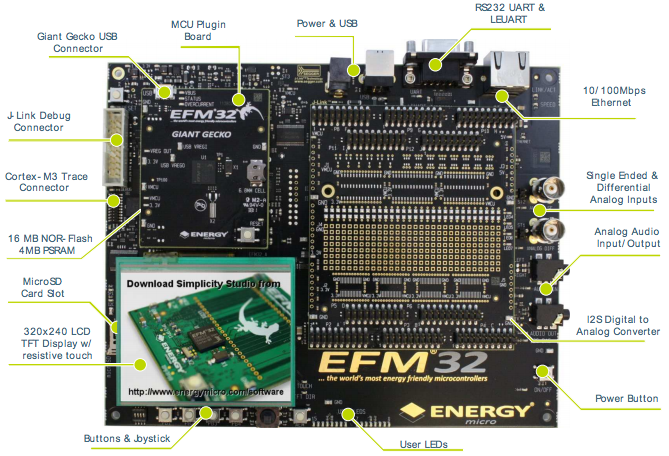
\includegraphics[scale=0.5]{figures/efm32gg-dk3750}
  \end{center}
  \caption{The Giant Gecko Development Kit - EFM32GG-DK3750 \cite{Labs2013_DK}}
  \label{fig:efm32gg-dk3750}
\end{figure}

\begin{figure}[H]
  \begin{center}
    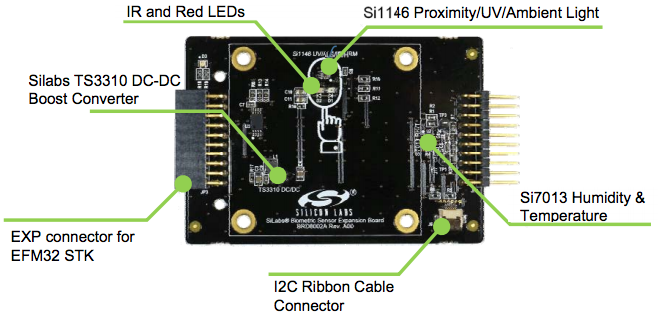
\includegraphics[scale=0.5]{figures/biometric-exp}
  \end{center}
  \caption{The Biometric-EXP Evaluation Board - BIOMETRIC-EXP-EVB \cite{Labs2014_BIO_EXP}}
  \label{fig:biometric-exp}
\end{figure}


\autoref{tab:hw:boards} summarizes the different hardware devices that are referred to throughout this report.
The original device-names are shortened in order to simplify reading.

\begin{table}[H]
  \begin{tabular}{l|l|l}
    \textbf{Product Name} & \textbf{Description} & \textbf{Short name} \\
    \hline
    EFM32GG & The Giant Gecko Microcontroller & \gecko \\
    EFM32GG-STK3700 & Giant Gecko Starter Kit & \texttt{STK} \\
    EFM32GG-DK3750 & Giant Gecko Development Kit & \texttt{DK} \\
    BIOMETRIC-EXP-EVB & Biometric Sensor Expansion Board & \texttt{BIO-EXP} \\
    \hline
  \end{tabular}
  \caption{Hardware devices}
  \label{tab:hw:boards}
\end{table}

\subsection{Peripherals}
\label{sub:peripherals}

\autoref{fig:efm32gg990_block_diagram} shows a block diagram of the Giant Gecko.
The Cortex-M3 and its memory can be found in the upper left corner, it can be seen from the diagram that the \gls{mcu} is connected to all other peripherals over a 32-bit bus.
This section will shortly introduce the peripherals that are relevant in this project, we will describe what they can be used for and why they are important, but we will not go into detail of how they work.
These details can be found in the Giant Gecko reference manual \cite{Labs}.

\begin{figure}[H]
\begin{center}
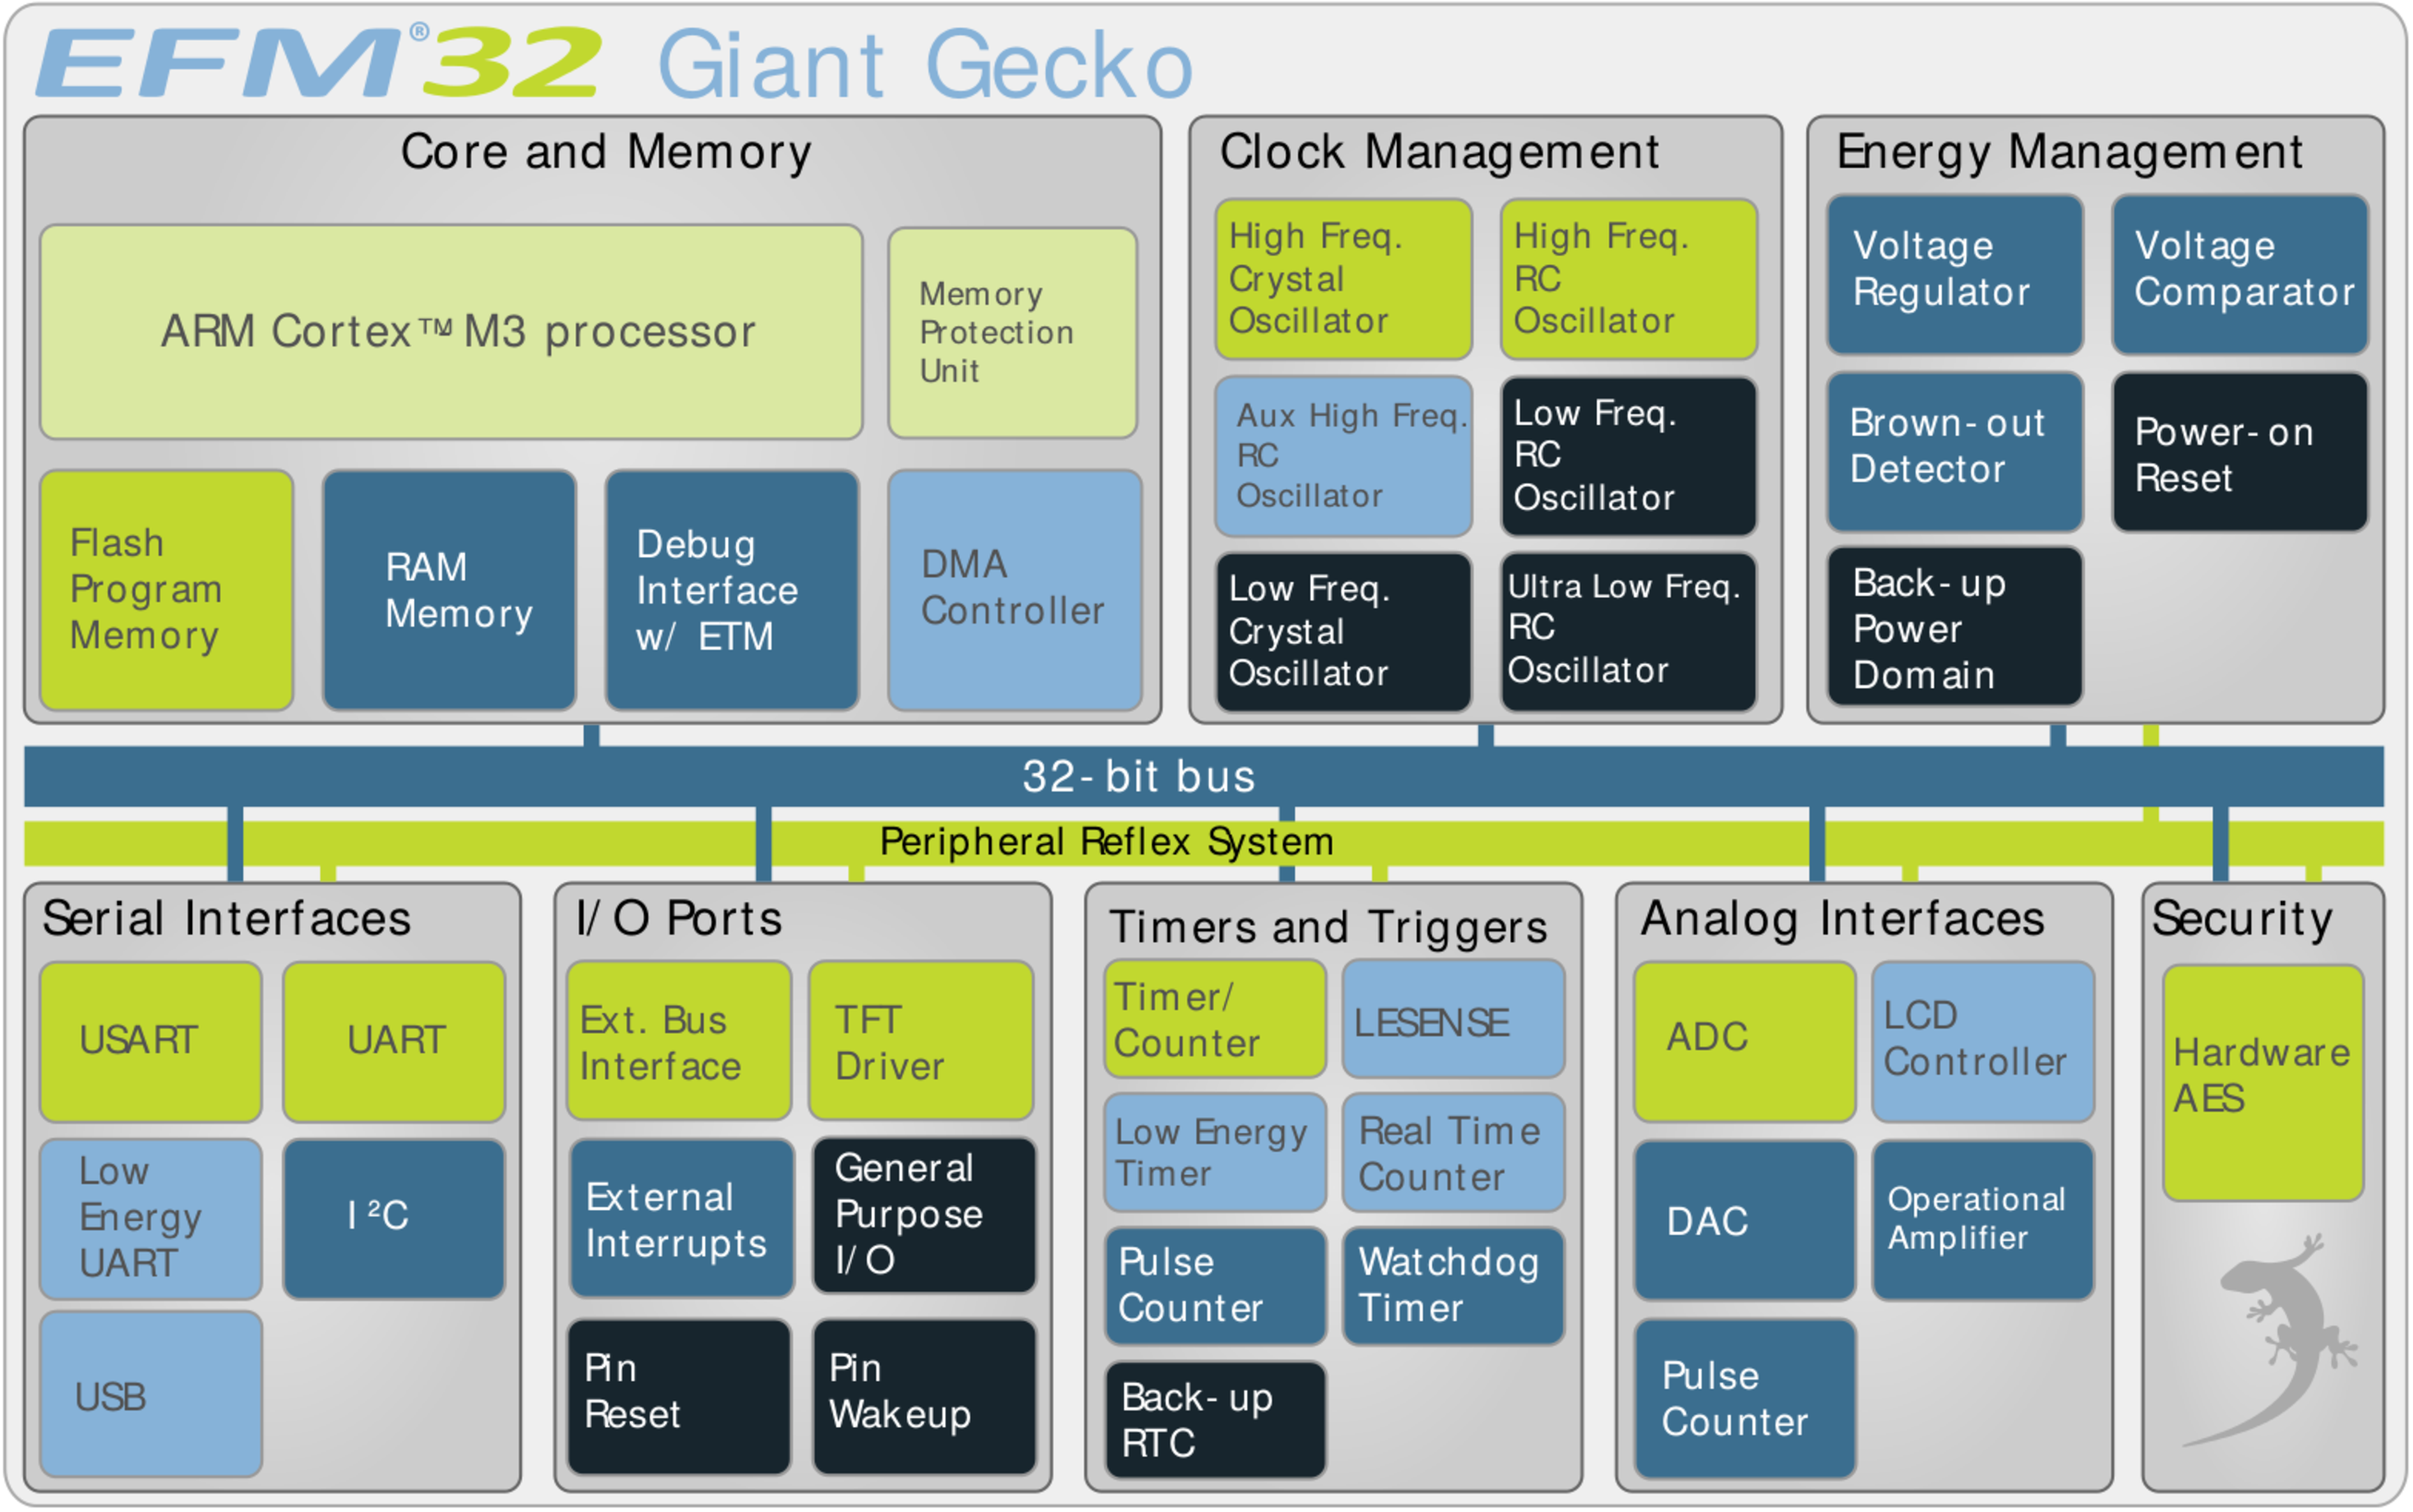
\includegraphics[width=0.8\textwidth]{figures/gg_block_diagram}
\end{center}
\caption{Giant Gecko block diagram \cite{Labs}.}
\label{fig:efm32gg990_block_diagram}
\end{figure}

Communication is important in every modern computing system, the {\gecko} supports a handful of different serial communication protocols through different peripherals.
The \gls{usart}, and the \gls{uart}, together with the \gls{i2c}, are serial protocols that allows for efficient communication between a high range of external devices.
Different areas of use can be e.g. reading and writing to SD memory cards or transferring data over a serial interface to a computer.
Peripherals like the \gls{usart} and the \gls{uart} can be used in combination with \gls{dma}, which is useful for energy constrained applications.
This combination makes it possible to implement applications that can gather data from a range of external sensors, and transfer or store it to other peripherals with minimal interaction from the \gls{cpu}.

\gls{gpio} is used for pin configuration and manipulation of the \gls{mcu} pins, and are often used in order to configure the pins that are required by other peripherals.
Simple Push Buttons and LEDs are configured with the \gls{gpio}, and e.g. the \gls{usart} needs to have configured at least two \gls{gpio} pins for both receiving and transmitting data.

Many applications are used to gather data by measuring different sensors and signals.
The \gls{adc} is a peripheral that is used to measure analog signals, like e.g. sound or light intensity, and convert them to digital signals.
Oppositely, the \gls{dac} can be used to convert digital signals back to e.g. analog sound signals.

Timers are another important peripheral type, the {\gecko} supports a number different timers that operate with different frequencies and at different energy levels.
The Timer peripheral is used to generate signals at specified frequencies.
These signals can be software interrupts to the \gls{cpu} or other peripherals, which in turn, without intervention from the \gls{cpu}, can be used to e.g. initiate a \gls{dma} transfer over \gls{uart} at timed intervals.
The \gls{rtc} is another timer that work at low energy levels which is useful for energy constraint applications.
